\documentclass{article}
\usepackage{amsmath}
\usepackage{amssymb}
\usepackage{graphicx}
\usepackage{float}
\usepackage{multirow}
\usepackage{verbatim}

\setlength{\parindent}{0em}
\setlength{\parskip}{1em}
\renewcommand{\arraystretch}{1.5}

\newcommand{\diff}{\mathop{}\!\mathrm{d}}
\newcommand{\prob}{\mathbb{P}}
\newcommand{\expect}{\mathbb{E}}

\title{Assignment 4}
\author{Joshua Hwang (44302650)}
\date{19 April}

\begin{document}
\maketitle

\section{Square root pdf}
\subsection{Determine $c$}
A pdf's total area must be equal to 1.
Thus we must ensure,
\begin{align*}
    \int_1^9 c\sqrt{x} \diff x &= 1 \\
    c \left[\frac{2}{3} x^{\frac{3}{2}}\right]_1^9 &= 1 \\
    \frac{2c}{3} \left[x^{\frac{3}{2}}\right]_1^9 &= 1 \\
    \frac{2c}{3} \left[9^{\frac{3}{2}} - 1^{\frac{3}{2}}\right] &= 1 \\
    \frac{2c}{3} \left[27 - 1\right] &= 1 \\
    \frac{52c}{3} &= 1 \\
    c &= \frac{3}{52} \\
\end{align*}

\subsection{Expectation of $X$}
We use the following,
\begin{align*}
    \int_1^9 xf(x) \diff x &= \frac{3}{52}\int_1^9 x\sqrt{x} \diff x \\
    &= \frac{3}{52} \left[\frac{2}{5}x^\frac{5}{2}\right]_1^9 \\
    &= \frac{6}{260} \left[9^\frac{5}{2} - 1\right] \\
    &= \frac{3}{130} \left[243 - 1\right] \\
    &= \frac{726}{130} \\
    &= 5.58 && \text{2 decimal places}
\end{align*}

\subsection{Explain the inverse-tranform method}
Let $F(x) = \int_\text{min}^x f(y) \diff y$. The inverse transform states,
$X = F^{-1}(U)$, where $U \sim U(0,1)$. We can verify this as follows,
\begin{align*}
    \prob(X \leq x) &= \prob(F^{-1}(U) \leq x) \\
    &= \prob(U \leq F(x)) \\
    &= F(x) \\
\end{align*}

Now that we have verified the inverse-transform method works we need to find
$F^{-1}(x)$.
\begin{align*}
    F(x) &= \int_1^x f(y) \diff y \\
    &= \frac{3}{52}\int_1^x \sqrt{y} \diff y \\
    &= \frac{3}{52}\frac{2}{3}\left[x^{\frac{3}{2}} - 1\right] \\
    &= \frac{1}{26}\left[x^{\frac{3}{2}} - 1\right] \\
    \left(26F(x) + 1\right)^{\frac{2}{3}} &= x
    && \text{Take the left hand side as the inverse} \\
    F^{-1}(x) &= \left(26U + 1\right)^{\frac{2}{3}} \\
\end{align*}

\verbatiminput{q1.py}

This gave us
\begin{verbatim}
The mean is: 5.586159189910373
\end{verbatim}

Which corresponds quite well to our calculations.

\section{Joint pmf}
\subsection{Marginal pmfs}
The marginal pmf for each $X$ and $Y$ is determined by,
\begin{align*}
    pmf(X) &= \sum_Y pmf(X, Y)
\end{align*}

Thus we produce,
\begin{center}
\begin{tabular}{ |c|c| }
    \hline
    $X$ & $\prob(X)$ \\
    \hline
    2 & 0.4 \\
    5 & 0.2 \\
    6 & 0.4 \\
    \hline
\end{tabular}
\end{center}

\begin{center}
\begin{tabular}{ |c|c| }
    \hline
    $Y$ & $\prob(Y)$ \\
    \hline
    0 & 0.4 \\
    1 & 0.2 \\
    2 & 0.2 \\
    3 & 0.2 \\
    \hline
\end{tabular}
\end{center}

\subsection{Independence}
A joint pmf has independent variables if and only if
\begin{align*}
    \prob(X_1=x_1, X_2=x_2...) = \prob(X_1=x_1) = \prob(X_2=x_2)... \\
\end{align*}
This is not the case since $\prob(X = 5, Y = 1) \neq \prob(X=5)
\neq \prob(Y=1)$.

\subsection{Covariance}
Covariance is defined as,
\begin{align*}
    Cov(X,Y) &= \expect(X - \expect X)(Y - \expect Y) \\
    Cov(X,Y) &= \expect XY - \expect X \expect Y
    && \text{Another representation} \\
\end{align*}

Since we have such a small sample size we manually determine this.
$\expect X = 4.2$, $\expect Y = 1.2$ and $\expect XY = 4.8$.

Thus the covariance is $-0.24$.

\section{Another joint pmf}
\subsection{Produce table}
We notice all values of $U$ and $V$ are already specified. Since they are
independent we can create a table for them with the information we have.
\begin{center}
\begin{tabular}{ c c|c c  }
    & & \multicolumn{2}{c}{$V$} \\
    & & 1 & -1\\
    \hline
    \multirow{2}{*}{$U$} & 1 & $\frac{1}{16}$ & $\frac{3}{16}$ \\
    & -1 & $\frac{3}{16}$ & $\frac{9}{16}$ \\
\end{tabular}
\end{center}

We can now create $X$ and $Y$.
We notice only two possible values are possible for $X$, 1 and -1. While
$Y$ has three, -2, 0 and 2. We take all four pairs of values of $U$ and $V$
from the table and calculate $X$ and $Y$ to put into the table below.
\begin{center}
\begin{tabular}{ c c|c c  }
    & & \multicolumn{2}{c}{$X$} \\
    & & 1 & -1\\
    \hline
    \multirow{3}{*}{$Y$} & 2 & $\frac{1}{16}$ & 0 \\
    & 0 & 0 & $\frac{6}{16}$ \\
    & -2 & $\frac{9}{16}$ & 0 \\
\end{tabular}
\end{center}

\subsection{Expectation and variance for $Y$}
Repeating the process from the last question we obtain,
$\expect X = \frac{10}{16} - \frac{6}{16} = \frac{1}{4}$.
Variance is obtained by,
\begin{align*}
    Var(X) &= \expect X^2 - (\expect X)^2 \\
    &= 1 - \frac{1}{16} && \text{$X^2$ is guaranteed 1} \\
    &= \frac{15}{16} \\
    \sqrt{Var(X)} &= 0.97 \\
\end{align*}

\subsection{Correlation coefficient}
The correlation coefficient is,
\begin{align*}
    \rho(X,Y) &= \frac{Cov(X,Y)}{\sqrt{Var(X)}\sqrt{Var(Y)}}
\end{align*}

We now find $Var(Y)$ using the same methods as before.
\begin{align*}
    \expect Y &= 2\frac{1}{16} - 2\frac{9}{16} = \frac{-16}{16} = -1 \\
    \expect Y^2 &= 4\frac{1}{16} + 4\frac{9}{16} = \frac{40}{16} = 2.5 \\
    Var(Y) &= \expect Y^2 - (\expect Y)^2 \\
    &= 2.5 - 1 = 1.5 \\
    \sqrt{Var(Y)} &= 1.22 \\
\end{align*}
 
We now find covariance,
\begin{align*}
    Cov(X,Y) &= \expect XY - \expect X \expect Y \\
    &= 2\frac{1}{16} - 2\frac{9}{16} + \frac{1}{4} \\
    &= -1 + \frac{1}{4} \\
    &= -\frac{3}{4} \\
\end{align*}

Now we determine the correlation coefficient,
\begin{align*}
    \rho(X,Y) &= \frac{Cov(X,Y)}{\sqrt{Var(X)}\sqrt{Var(Y)}} \\
    &= \frac{-\frac{3}{4}}{0.97 \times 1.22} \\
    &= -0.63 \\
\end{align*}

\section{Continuous joint distribution}
\subsection{Create pdf}
All points within the triangle are equally likely thus we represent our
pdf as a constant piecewise function.
\begin{align*}
    f(x,y)
    &=
    \begin{cases}
        c & (x,y) \in \text{triangle} \\
        0 & (x,y) \notin \text{triangle}
    \end{cases} \\
\end{align*}

We find what $c$ has to be to ensure $\iint f \diff x \diff y = 1$.
Note: the bounds of our integral are written in terms of $x$, the swapped
version is also applicable (in terms of $y$).
\begin{align*}
    \int_0^1 \int_0^x f(x,y) \diff y \diff x &= 1 \\
    c \int_0^1 \int_0^x 1 \diff y \diff x &= 1 \\
    c \frac{1}{2} &= 1 \\
    c &= 2 \\
\end{align*}

Thus our pdf is 
\begin{align*}
    f(x,y)
    &=
    \begin{cases}
        2 & (x,y) \in \text{triangle} \\
        0 & (x,y) \notin \text{triangle}
    \end{cases} \\
\end{align*}

\subsection{Marginal pdf}
The marginal pdf for a contiunous function is much the same to the discrete
case.
\begin{align*}
    f_Y(y) &= \int_y^1 f(x,y) \diff y \\
    &= 2(1-y) \\
\end{align*}

\subsection{Expectation of $Y$}
Expectation can be calculated as follows,
\begin{align*}
    \expect Y &= \int_0^1 y f_Y(y) \diff y \\
    &= 2 \int_0^1 y - y^2 \diff y \\
    &= 2 \left(\frac{1}{2} - \frac{1}{3}\right) \\
    &= \frac{1}{3}
\end{align*}

\section{Another continuous join distribution}
\subsection{Find $c$}
We know the integral must give 1 so,
\begin{align*}
    \int_0^1 \int_0^1 f_{X,Y}(x,y) \diff x \diff y &= 1 \\
    \int_0^1 \int_0^1 cxy \diff x \diff y &= 1 \\
    c \int_0^1 x \diff x \int_0^1 y \diff y &= 1 \\
    c \frac{1}{4} &= 1 \\
    c &= 4 \\
\end{align*}

\subsection{Are $X$ and $Y$ independent?}
Yes they are independent to show this we first show the marginal pdfs
for the above.
\begin{align*}
    f_X(x) &= \int_0^1 f_{X,Y}(x,y) \diff y \\
    &= 4x\int_0^1 y \diff y \\
    &= 2x \\
\end{align*}

The same will apply for the $f_Y(y)$ case.

We know a joint pdf has independent variables iff
\begin{align*}
    f(x,y) &= f_X(x)f_Y(y) \\
    4xy &= 4xy \\
\end{align*}

\subsection{Calculate probability}
Since maximum of $Y$ is 1 we know all $X>0.5$ is valid. For $X<0.5$ the
inequality needs to be checked. In this way we are able to split our joint
distribution up. Probabilities are calculated by integrating the pdf.
\begin{align*}
    \prob(2X>Y) &= \iint_{2x>y} f(x,y) \diff x \diff y \\
    &= 4 \int_0^1 y \diff y \int_{0.5}^1 x \diff x
    + 4 \int_0^{0.5} x \int_0^{2x} y \diff y \diff x \\
    &= (1 - 0.25) + 8 \int_0^{0.5} x^3 \diff x \\
    &= (1 - 0.25) + 2 \frac{1}{16} \\
    &= (1 - 0.25) + \frac{1}{8} \\
    &= \frac{7}{8} \\
\end{align*}

\section{10 random numbers}
\subsection{$M$ as $X_1, X_2 ... X_{10}$}
\begin{align*}
    M &= max\{X_1, X_2 ... X_{10}\}
\end{align*}

(Yeah, don't know what else to put here)

\subsection{Determine pdf and expectation}
It is easier to work with $\prob$ and $F$ to begin with.
\begin{align*}
    F(m) &= \prob(max\{X_1, X_2... X_{10}\} \leq m) \\
    &= \prob(X_1 \leq m \cap X_2 \leq m ... X_{10} \leq m) \\
    &= \prob(X_1 \leq m) \prob(X_2 \leq m) ... \prob(X_{10} \leq m) \\
    &= F_{X_1}(m) F_{X_2}(m) ... F_{X_{10}}(m) \\
\end{align*}

To get the pdf we will have to differentiate the following. Luckily
$\forall X_i \sim U(0,1)$ so $f_{X_i}(m) = 1$. Additionally, $F_{X_i}(m) = m$.
In total our final pdf comes
to be
\begin{align*}
    f(m) &= \sum_{i=1}^{10} f_{X_i}(m) \prod_{j \neq i} F_{X_j}(m) \\
    &= \sum_{i=1}^{10} \prod_{j \neq i} m \\
    &= 10m^9 \\
\end{align*}

Funnily enough this matches a $F(m) = m^{10}$ the probability that all 10
are below a certain number. The derivation process completed above was
kinda useless.

The expectation of $M$ can now be found,
\begin{align*}
    \int_0^1 m f(m) \diff m &= 10 \int_0^1 m^10 \diff m \\
    &= \frac{10}{11} \\
\end{align*}

\section{Functions of random variables}
We take the probability of $Y$ and work from there,
\begin{align*}
    \prob(Y \leq y) &= \prob(X \leq \ln(y)) \\
    &= F_X(\ln(y)) \\
\end{align*}

Thus our pdf is $f_Y = \frac{1}{y} f_X(\ln(y)) = \frac{1}{y\sqrt{2\pi}}e^{-0.5(\ln(y))^2}$.
\begin{figure}[H]
    \centering
    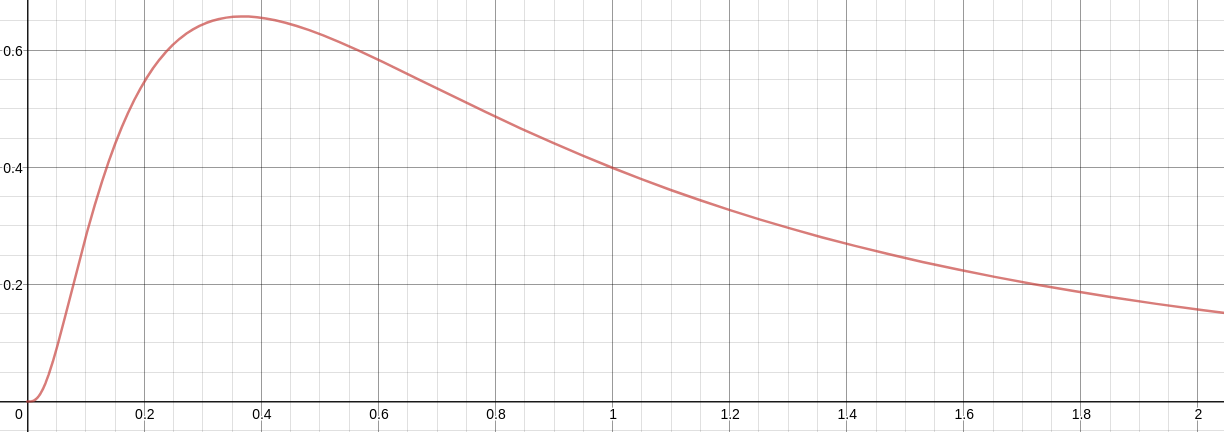
\includegraphics[width=5in]{graph.png}
\end{figure}

\section{Simulation}
I used the following to simulate the snakes and ladders game with a single die.
\verbatiminput{q8.py}

The following result was obtained.
\begin{verbatim}
The mean is: 7.4
\end{verbatim}

The graph below is the estimated pmf for the snake and ladder game.
\begin{figure}[H]
    \centering
    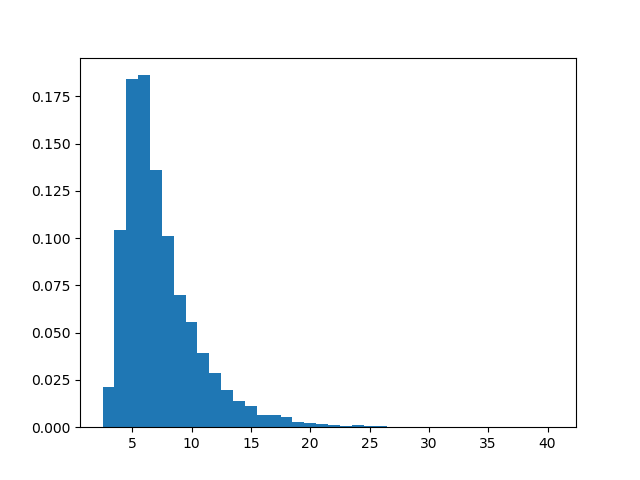
\includegraphics[width=5in]{graph2.png}
\end{figure}

\end{document}
